% ---------------------------------------------------------------------------
% Ablation study. Generated by ablation/section_numbers.py from
% ablation/ablation_section_template.tex and the files in ablation/results/:
% edit the template, not the numbers. Needs \usepackage{graphicx}; the figures
% are in ablation/figures/.
% ---------------------------------------------------------------------------
\subsection{Ablation Study}
\label{sec:ablation}

To measure what each component contributes, we removed or replaced one component at a time while keeping the data, splits, seeds, hyperparameters and metrics fixed. The ablations run against the released code through a harness that imports the application unmodified and only wraps, subclasses or monkeypatches the component under test (\texttt{ablation/} in the repository). Where the implementation differs from Section~\ref{sec:methodology}, we ablate the implementation and state the difference.

\subsubsection{Protocol}
\emph{Data.} Adult (OpenML~1590; label \texttt{>50K} coded as~1), Credit Card Fraud (OpenML~1597; 29 features, without the \texttt{Time} column) and California Housing (scikit-learn; target in \$100k) pass through the application's \texttt{AutoPreprocessor} with its default settings (SMOTE off), exactly as in the UI. After its de-duplication, its 80/20 split (stratified for classification) yields 9{,}758, 55{,}133 and 4{,}128 test rows. \texttt{fit\_transform} fits the outlier caps, skew transforms, imputer, encoder (target encoding uses the full label vector) and feature selector on all rows before splitting; only the scaler is fitted on the training partition. Every experiment is repeated on five splits (seeds 0--4) and reported as mean$\pm$standard deviation.

\emph{Models and timing.} Brute force trains every model returned by \texttt{ModelTrainer.get\_supported\_models()} (9 classifiers, 12 regressors) with the application's default hyperparameters; the code contains no ensemble or stacking model. All runs are single-threaded on a 4-vCPU container (Python~3.11, scikit-learn~1.3.2, XGBoost~2.0.3, SHAP~0.46.0), so times are comparable with each other but not with Table~\ref{tab:latency}.

\emph{Recommendation engine (A).} \emph{Full} retrieves $k{=}3$ chunks of \texttt{ml\_rules.txt}, adds meta-learning priors from the workspace store---seeded through the real \texttt{WorkspaceManager} with completed sessions of the two other benchmarks---and filters the LLM output with the UI's name matcher. \emph{w/o RAG} empties the retrieved context, \emph{w/o Meta-learning} passes no workspaces, and \emph{w/o Fuzzy matcher} sends the raw names to \texttt{ModelTrainer}. The implemented matcher performs exact, case/space-normalised and substring matching against the supported-model list and falls back to a default selection when nothing matches; the code contains no Levenshtein distance or threshold~$\tau$. The Groq model hard-coded in the advisor (\texttt{llama-3.3-70b-versatile}) is no longer served, so the unmodified advisor (\emph{As shipped}) always returns its fallback; all other rows substitute \texttt{openai/gpt-oss-120b} at the application's temperature (0.3) with the prompt, retriever, parser and fallbacks unchanged. Each configuration was queried <<n_calls_per_cfg>> times per dataset, and each selected set was scored on all five splits. Because a fit is deterministic given its split, the selected models' metrics are read from the brute-force run of the same split, while the name-to-model dispatch still runs through \texttt{ModelTrainer.run\_selected\_models}.

\emph{Preprocessing (B).} \emph{Stateful} serving saves the fitted \texttt{AutoPreprocessor}, reloads it and calls \texttt{transform} on raw test rows before \texttt{predict}, as \texttt{/predict} does; \emph{stateless} serving fits a new \texttt{AutoPreprocessor} on each serving batch of 1, 16, 256 or all test rows. Both are compared with the \emph{offline} predictions on the \texttt{fit\_transform} output for the same rows, which underlie every reported metric. Batches of 1--256 rows are cut from a random 1{,}024-row stream; for Credit Card Fraud, where such a stream holds about two frauds, the stream is enriched with all test frauds. We also send reordered columns, an unseen category and a missing column, and call the real \texttt{/predict} endpoint through FastAPI's \texttt{TestClient}.

\emph{SHAP (C).} The application's \texttt{SHAPExplainer} (first 200 test rows; 50-row background for \texttt{KernelExplainer}) runs with its keyword routing and float32 cast (\emph{Full}), with the router forced to \texttt{TreeExplainer} or to \texttt{KernelExplainer}, and without the cast, for Random Forest, XGBoost, Gradient Boosting, Logistic Regression/Ridge, SVM and KNN; each job runs in its own process with a 300\,s limit.

<<TABLE>>

\begin{figure}[t]
\centering
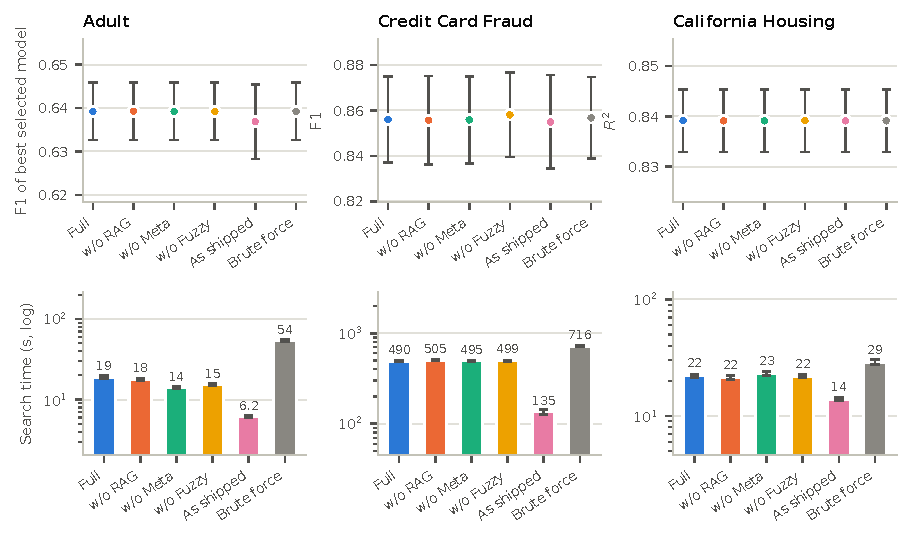
\includegraphics[width=\textwidth]{figures/fig_ablation_rag.pdf}
\caption{Recommendation-engine ablation (mean$\pm$std over five splits; 10 LLM calls per configuration). Top: F1 (classification) or $R^2$ (regression) of the best model in the selected set. Bottom: search time, i.e.\ LLM latency plus training of the selected models on one thread (log scale).}
\label{fig:abl-rag}
\end{figure}

\subsubsection{Recommendation Engine}
All <<n_llm_calls_substitute>> calls to the substitute LLM returned parseable JSON in which every name was in the supported list (Valid = 100\,\% in every row of Table~\ref{tab:ablation}), with and without retrieved context: the prompt's explicit list of permitted models, not retrieval, keeps the names valid. Bypassing the name matcher therefore caused no runtime failure. The matcher only acts on names this LLM never produced: of <<probe_n>> spellings typical of LLM output it maps <<probe_mapped>> (only <<probe_exact>> would train without it), silently accepts the paper's hallucination example \texttt{RandomForestClassifierRegressor} as Random Forest, and leaves library class names such as \texttt{XGBClassifier}, \texttt{SVC} and \texttt{KNeighborsClassifier} unmatched.

On every split and every call, each configuration's selected set contained a model that reached the brute-force optimum of the application's selection metric (Accuracy or RMSE; the largest shortfall over all calls and splits is <<max_metric_gap_vs_bf>>), so the quality columns of the recommendation rows coincide with brute force (Fig.~\ref{fig:abl-rag}). The engine's benefit is the compute it saves by skipping slow models: Full needs <<adult_red_train>>\,\%, <<credit_red_train>>\,\% and <<california_red_train>>\,\% less training time than brute force on Adult, Credit and California. On Credit the saving is small because the LLM recommends Gradient Boosting in <<credit_gb_rate>>\,\% of the calls, and on that dataset it is both the slowest model (<<credit_gb_time>>\,s per fit) and the least accurate one (AUC <<credit_gb_auc>>). Removing retrieval leaves the quality unchanged and saves <<rag_latency_delta>>\,s of latency and <<rag_token_delta>> tokens per call. The hard-coded fallback of the shipped advisor (XGBoost and Random Forest, plus Linear Regression for regression), which involves no LLM at all, is the cheapest configuration (<<ship_red_min>>--<<ship_red_max>>\,\% less training time) and loses <<adult_ship_acc_drop>> accuracy on Adult and nothing on the other two datasets.

Meta-learning never activated. \texttt{find\_similar\_workspaces} accepts a prior session of the same task whose row count is within 50\,\% or whose column count is within 30\,\% of the new dataset's; no pair of the three benchmarks qualifies, so the Full and w/o Meta-learning prompts are identical and their differences in Table~\ref{tab:ablation} are LLM sampling noise. Even a prior session on the same dataset is found only for classification: for regression the UI compares the stored task type \texttt{"Regression"} with \texttt{"regression"} and never records a best model (<<repo_reg_ws_best>> of the <<repo_reg_ws>> regression workspaces in the repository have one). Injecting a same-dataset prior for Adult and Credit (supplementary run, \texttt{results/rag\_summary.csv}) changed the recommended sets but not their quality.

\begin{figure}[t]
\centering
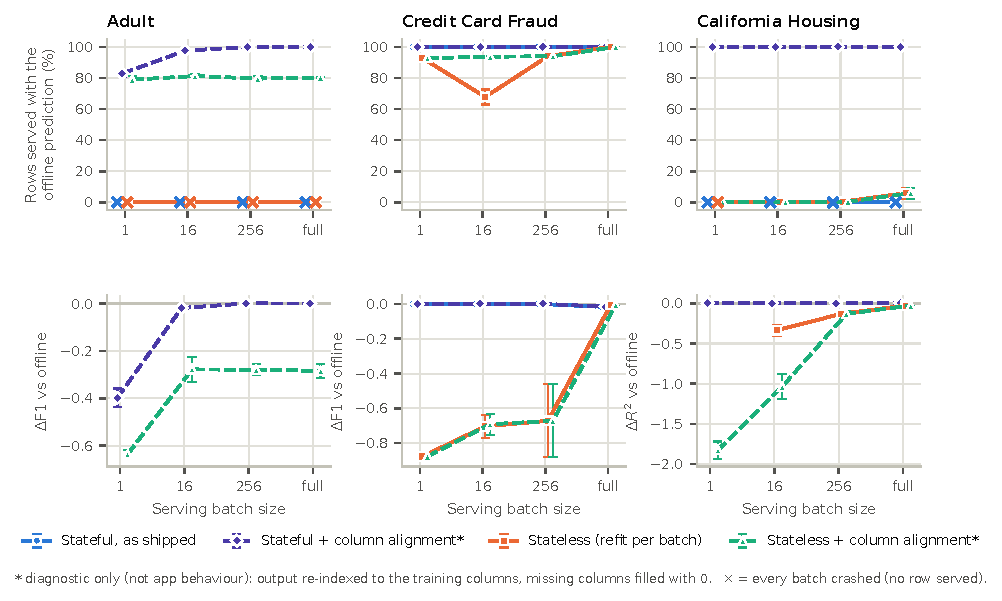
\includegraphics[width=\textwidth]{figures/fig_ablation_preprocessing.pdf}
\caption{Serving the XGBoost model on raw test rows. Top: share of rows whose served prediction equals the offline prediction; $\times$ marks configurations in which every batch crashed. Bottom: change in F1 or $R^2$ relative to the offline predictions on the rows that were served. Dashed lines re-index the transformed batch to the training columns (a diagnostic, not application behaviour).}
\label{fig:abl-preproc}
\end{figure}

\subsubsection{Stateful Preprocessing}
The serialized preprocessor does not reproduce \texttt{fit\_transform}: its \texttt{transform} skips the outlier caps, skew transforms and feature selection, and one-hot encodes each request with \texttt{pd.get\_dummies}. On Adult and California the columns removed by the selector (capital-gain, capital-loss and native-country; AveBedrms) reappear at serving time, so stateful serving as shipped fails on every batch of every size, and \texttt{/predict} answers HTTP~500 to every request---unperturbed, with reordered columns, with an unseen category or with a missing column (Table~\ref{tab:ablation}, Fig.~\ref{fig:abl-preproc}). On Credit the schema matches, but all <<credit_mismatch_feats>> features differ from the training representation for rows beyond the fitted caps; the served predictions still equal the offline ones for <<credit_stream_stateful_agree>>\,\% of the fraud-enriched stream and <<credit_full_stateful_agree>>\,\% of the full test set (F1 <<credit_full_off_f1>> offline vs.\ <<credit_full_srv_f1>> served). The Credit endpoint answers unperturbed requests (HTTP~200) but returns HTTP~500 for reordered columns and, after silently retrying on the raw input, for a missing column.

Refitting per batch (stateless) is worse wherever it runs. On Credit it collapses fraud detection: at batch sizes 1--256, F1 falls to at most <<credit_stateless_f1_small_max>> and only <<credit_stateless_agree_small>>\,\% of the predictions agree with stateful serving; F1 recovers (<<credit_stateless_full_f1>>) only when one batch is the entire test set. On California it crashes on every single-row batch and on <<ca_stateless_crash16>>\,\% of the 16-row batches, and $R^2$ falls from <<ca_off_r2>> to <<ca_stateless_r2_256>> at batch size 256 (<<ca_stateless_r2_full>> on the full test set); on Adult it crashes on every batch. Re-indexing the output to the training columns (diagnostic only) lets stateful serving reproduce at least <<tree_aligned_min_agree>>\,\% of the tree models' offline predictions for batches of 256 rows or more, but single-row requests on Adult still agree with the offline predictions for only <<adult_aligned1_agree>>\,\% of the rows (F1 <<adult_off_f1>>$\rightarrow$<<adult_aligned1_f1>>), because \texttt{get\_dummies(drop\_first=True)} emits no one-hot column for a single row. Where \texttt{/predict} succeeds (Credit), a single-row request takes a median <<lat_credit_min>>--<<lat_credit_max>>\,ms in-process, including reloading the workspace, the model file and the <<pipeline_pkl_credit_mb>>\,MB pipeline file (which stores the processed training and test data) on every request; the model itself predicts in about <<model_only_ms>>\,ms.

\begin{figure}[t]
\centering
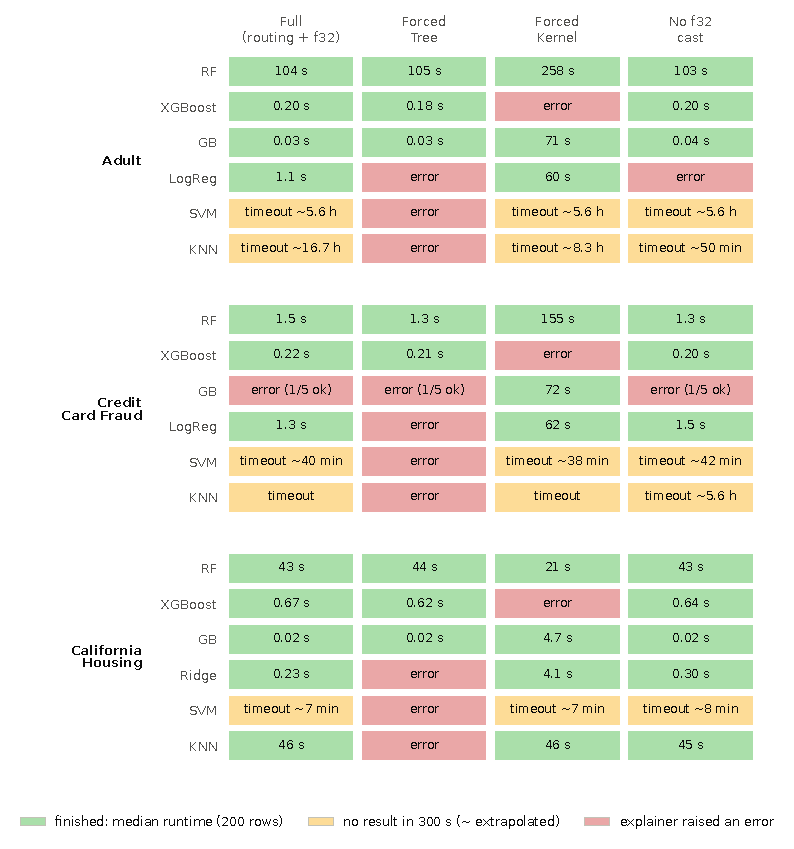
\includegraphics[width=0.82\textwidth]{figures/fig_ablation_shap.pdf}
\caption{SHAP ablation per model family (median runtime for 200 test rows over the five splits; ``timeout'' = no result within 300\,s, with the time to completion extrapolated from the rows finished; parentheses give the number of successful splits when it is not all or none).}
\label{fig:abl-shap}
\end{figure}

\subsubsection{SHAP Routing and Pre-Casting}
With the shipped routing, SHAP values were produced for <<shap_adult_full_ok>>, <<shap_california_full_ok>> and <<shap_credit_full_ok>> of six model families on Adult, California and Credit (mean over splits; Fig.~\ref{fig:abl-shap}). SVM never finishes within 300\,s (extrapolated <<svm_extrap_adult_h>>\,h on Adult, <<svm_extrap_credit_min>>\,min on Credit and <<svm_extrap_ca_min>>\,min on California), KNN exceeds the limit on Adult and Credit, and on Credit \texttt{TreeExplainer} fails its additivity check for Gradient Boosting on <<credit_gb_tree_fail>> of <<credit_gb_tree_n>> splits (SHAP sum $<<gb_additivity_sum>>$ vs.\ model output $<<gb_additivity_out>>$), with or without the cast. Forcing \texttt{TreeExplainer} crashes on every non-tree model, as expected. Forcing \texttt{KernelExplainer} is much slower than the specialised explainers where it finishes (e.g., Gradient Boosting on Adult <<adult_gb_tree_s>>\,s$\rightarrow$<<adult_gb_kernel_s>>\,s, Logistic Regression <<adult_lr_lin_s>>\,s$\rightarrow$<<adult_lr_kernel_s>>\,s), fails for XGBoost because SHAP~0.46 cannot set XGBoost's read-only \texttt{feature\_names\_in\_}, and still times out on SVM and KNN; for the deep California Random Forest it is, counter-intuitively, faster than \texttt{TreeExplainer} (<<ca_rf_kernel_s>>\,s vs.\ <<ca_rf_tree_s>>\,s). Removing the float32 cast changes one outcome: on Adult, whose one-hot columns are Boolean, \texttt{LinearExplainer} fails because the mixed frame becomes an object array on which \texttt{np.cov} raises (\texttt{'float' object has no attribute 'shape'}). This is a dtype error rather than the Boolean-subtraction overflow described in Section~\ref{sec:shap}, and none of the successful runs returned NaN values. The cast also has a cost: on Adult, \texttt{KernelExplainer} finished <<knn_rows_cast>> rows of KNN within 300\,s with the cast and <<knn_rows_nocast>> without it, and its peak memory grew from <<knn_mem_nocast_gb>> to <<knn_mem_cast_gb>>\,GB.

\begin{figure}[t]
\centering
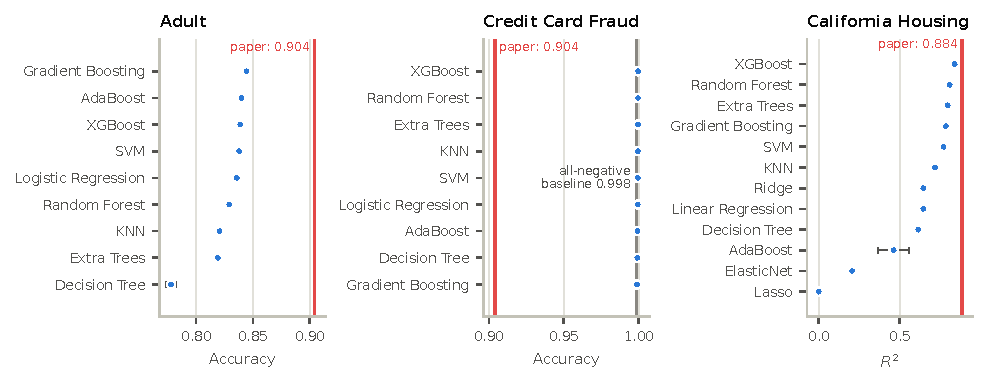
\includegraphics[width=\textwidth]{figures/fig_measured_vs_claimed.pdf}
\caption{Brute-force results of every supported model (mean$\pm$std over five splits) against the values reported in Tables~\ref{tab:classification} and~\ref{tab:regression}. The code contains no ensemble model, so the ``AI-selected ensemble'' cannot be evaluated.}
\label{fig:abl-claims}
\end{figure}

\subsubsection{Consistency with the Headline Results}
The ablation does not reproduce the headline numbers reported earlier in this paper (Fig.~\ref{fig:abl-claims}). (i)~The best Adult accuracy over all nine supported models is <<adult_best_acc>>$\pm$<<adult_best_acc_std>> (<<adult_best_acc_model>>), not 0.904; the preprocessor's IQR capping turns capital-gain and capital-loss into constants, which the selector then removes. On Credit, every model's accuracy (<<credit_acc_min>>--<<credit_acc_max>>) lies near the all-negative baseline (<<credit_majority_acc>>), so an accuracy of 90.4\,\% would be far below that baseline; the best fraud-class F1 is <<credit_best_f1>> (<<credit_best_f1_model>>). (ii)~The best California $R^2$ is <<california_best_r2>>$\pm$<<california_best_r2_std>> (<<california_best_r2_model>>; RMSE \$<<california_best_rmse_usd>>), not 0.884. (iii)~The recommendation engine saves <<red_train_min>>--<<red_train_max>>\,\% of the training time of brute force, not 86.4\,\%, and none of the saving comes from meta-learning, which never activated. (iv)~\texttt{/predict} does not serve the Adult or California models at all, and it answers Credit requests in a median <<lat_credit_min>>--<<lat_credit_max>>\,ms rather than 12.4\,ms. The claims of hallucination-free selection, exact online--offline parity and 100\,\% SHAP routing success are not supported by the current code either: names are valid because of the prompt and, today, because of the hard-coded fallback; all fitted steps except the scaler see the test rows, and the serving path does not replay capping, skew transforms, feature selection or one-hot encoding; and routing succeeds for <<shap_full_rate_min>>--<<shap_full_rate_max>>\,\% of the model families within 300\,s.

\paragraph{Threats to validity.} The recommendation rows use a substitute LLM; a model that hallucinates more would make the matcher's limited coverage matter. Library versions follow the paper's stated scikit-learn~1.3 and XGBoost~2.0, whereas the unpinned \texttt{requirements.txt} installs newer versions today. Timings are single-threaded. Credit Card Fraud is the OpenML variant without \texttt{Time}. Adult's label was coded 0/1 because with the original string label XGBoost fails in the application's pipeline and F1 cannot be computed. SMOTE was left at its default (off).
